\section{Персистентные гомологии}
О персистентных гомологиях можно думать как об адаптации понятия гомологии к облаку точек. 

Имея облако точек $X$, существует много способов построения симплициальных комплексов по нему. Например, задав некоторый $\tau > 0$, можно рассматривать не просто точки, но и их окрестности с радиусом $\tau$. Тогда можно рассматривать следующую структуру: подмножество $\sigma \subset X$ будет симплексом, если пересечение окрестностей точек из $\sigma$ будет непусто. Тогда симплициальным комплексом, построенным по облаку точек, будет совокупность таких симплексов. Такой симплициальный комплекс называется \text{\it комплексом Чеха} $\Cech_\tau(X)$. 

На комплекс Чеха можно взглянуть с другой стороны: если данные действительно хорошо описывают некоторый топологический объект, который как бы стоит за этими данными, то, подобрав хороший радиус $\tau$, объединение полученных окрестностей будет гомотопически эквивалентно этому объекту. А так как все шары выпуклы, то объединение окрестностей будет гомотопически эквивалентно нерву данного покрытия. А значит, по лемме о нерве, сам нерв будет гомотопически эквивалентен топологическому объекту, который описывается данными. И комплекс Чеха как раз и является нервом покрытия. 

Но на практике оказывается, что комплекс Чеха очень сложно посчитать. Поэтому существует другой способ построения симплициального комплекса по облаку точек, более эффективный с точки зрения вычислений: зафиксировав $\tau$, подмножество $\sigma \subset X$ будет симплексом, если $\forall i,j \in \sigma: \rho(i,j) < \tau$. Симплициальным комплексом будет совокупность таких симплексов. Полученный симплициальный комплекс называется \text{\it комплексом Вьеториса—Рипса}(или просто {\it комплексом Рипса}) $\Rips_\tau(X)$.

\medskip
\begin{algorithm}[H]
	\small
	\SetAlgoLined
	\KwData{Облако точек $X$, вещественное число $\alpha > 0$. }
	\KwResult{Симплициальный комплекс Вьеториса—Рипса}
	Для каждой точки $x$ строим её $\alpha$-окрестность $B_\alpha(x)$;
	
	$i = 1$;
	
	\While{$i+1$ окрестностей попарно имеют непустое пересечение}{
		
		строим $i$-ый симплекс на соответствующих вершинах;
		
		$i \leftarrow i+1$; 
	}
	\caption{Алгоритм построения комплекса Вьеториса—Рипса}
\end{algorithm}
\medskip

То есть, вместо рассмотрения пересечений шаров, как это было в случае комплекса Чеха, рассматривают попарные расстояния между точками. Очевидно, такой подход более эффективен с вычислительной точки зрения, более того, его можно обобщить на общий случай конечного метрического пространства, и даже, более общо, на случай произвольного конечного множества с симметрической функцией.

Комплексы Чеха и Рипса связаны между собой: для облака точек $X \subset \mathbb{R}^d$ они имеют одинаковый 1-остов. Более того, справедливо следующее соотношение:
\[
	\Rips_\tau(X) \subseteq \Cech_\tau(X) \subseteq \Rips_{2\tau}(X).
\]

На рис. \ref{complexes} изображены комплексы Чеха и Рипса.

\begin{figure}[!htbp]
	\begin{center}
		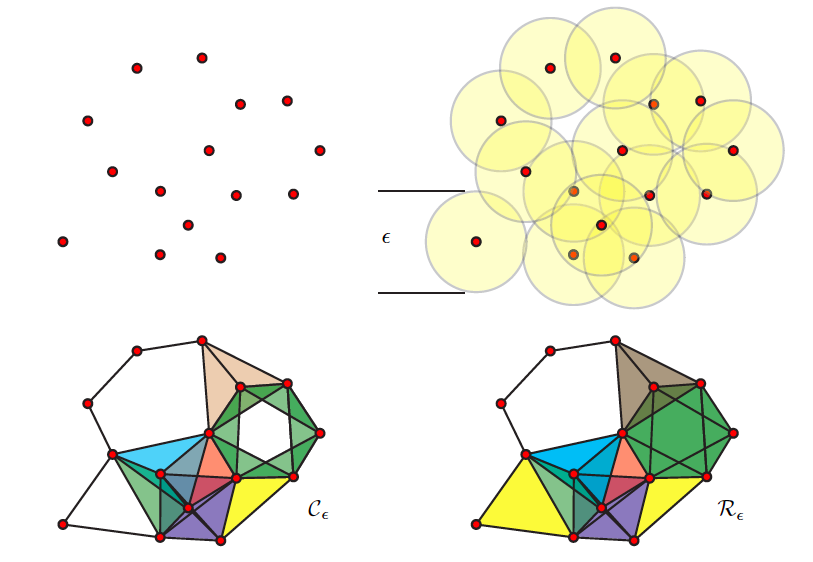
\includegraphics[width=0.75\textwidth]{complexes.png}\\
		\caption{Комплексы Чеха и Вьеториса—Рипса}
		\label{complexes}
	\end{center}
\end{figure}

Везде выше параметр $\tau$ был зафиксирован, но его можно изменять. Вслед за этим будут меняться и симплициальные комплексы, построенные с учетом $\tau$. {\it Фильтрацией симплициального комплекса $K$} называют вложенное семейство подкомплексов $ (K_\tau)_{\tau \in T} $, где $ T \subseteq \mathbb{R} $, такое, что если $ \tau < \tau^{'} $, то $ K_\tau \subseteq K_{\tau^{'}} $. Пример такой фильтрации изображен на рис. \ref{ripsfilt}, где изображения фильтрация симплициальных комплексов Рипса $\Rips_\tau(X)$.

\begin{figure}[!htbp]
	\begin{center}
		
\includegraphics[width=0.75\textwidth]{filtration.png}\\
		\caption{Фильтрация Рипса}
		\label{ripsfilt}
	\end{center}
\end{figure}

Имея фильтрацию $(K_\tau)_{\tau \in T}$, можно отслеживать изменение $H_k(K_\tau)$ с ростом $\tau$: могут появляться новые компоненты связности, уже существующие могут объединяться в одну компоненту, могут появляться циклы и "пустоты", соответствующие $1$ и $2$ группе гомологий. 
\begin{definition}
	$k$-ыми устойчивыми гомологиями фильтрованного комплекса $ (K_\tau)_{\tau \in T} $ называют  проиндексированное семейство абелевых групп $H_n(T) = \{ (H_n(K_\tau))_{\tau \in T} $ вместе с семейством гомоморфизмов $ (H_n(K_\tau) \to H_n(K_\tau^{'}))_{\tau \leq \tau^{'}} \}$.
\end{definition}
Такое семейство абелевых групп вместе с морфизмами на самом деле является примером  персистентного $\mathbb{Z}$-модуля: {\it персистентным $R$-модулем} $(A_*, x) $ называют последовательность $R$-модулей и гомоморфизмов между ними (над целочисленной временной шкалой $\mathbb{Z}_{\geq0}$).
\begin{center}
	\begin{tikzcd}[cells={nodes={minimum height=2em}}]
	A_0 \arrow[r, "x"] & A_1 \arrow[r,"x"]  &  A_2 \arrow[r,"x"] &  A_3 \arrow[r, "x"] & ... 
	\end{tikzcd}
\end{center}
Основная теорема про персистентные модули -- это структурная теорема. По аналогии с обычными модулями, она формулируется в терминах {\it конечнопорожденного} модуля устойчивости, т.е. такого модуля $(A_*, x)$, у которого существует конечный набор $a_1, ..., a_k \in A_*$ элементов, что любой элемент $a \in A_*$ можно выразить в виде линейной комбинации элементов вида $x^sa_r = x \circ ... \circ x(a_r)$.  Для ее формулировки понадобится еще пару определений: если $0 \leq j < s$, то {\it интервальным модулем устойчивости $I_{[j,s)}$} называют модуль устойчивости вида
\begin{center}
	\begin{tikzcd}[cells={nodes={minimum height=2em}}]
	0 \arrow[r] & ... \arrow[r]  &  0 \arrow[r] &  \underset{j}{R} \arrow[r, "id_R"] &  \underset{j+1}{R} \arrow[r, "id_R"] &
	... \arrow[r, "id_R"] & \underset{s-1}{R} \arrow[r, "0"] & \underset{s}{0} \arrow[r] & ... 
	\end{tikzcd}
\end{center}
Аналогично определяется бесконечный интервальный модуль $I_{[j, \infty)}$
\begin{center}
	\begin{tikzcd}[cells={nodes={minimum height=2em}}]
	0 \arrow[r] & ... \arrow[r]  &  0 \arrow[r] &  \underset{j}{R} \arrow[r, "id_R"] &  \underset{j+1}{R} \arrow[r, "id_R"] &
	... \arrow[r, "id_R"] & R \arrow[r, "id_R"] &  ... 
	\end{tikzcd}
\end{center}
Можно определить прямую сумму персистентных модулей: $ (A_*, x) \oplus (B_*, x) = ((A_* \oplus B_*), x) $, где $(A_* \oplus B_*)_j = A_j \oplus B_j$, а $x$ действует на каждом из слагаемых по отдельности.
\begin{theorem*}[об интервальном разложении] Пусть $R$ -- произвольное поле, а $(A_*, x)$ -- конечнопорожденный персистентный $R$-модуль. Тогда $(A_*, x)$ имеет единственное с точностью до перестановки слагаемых представление в виде прямой суммы конечного числа интервальный модулей:
	\[
		(A_*, x) \simeq \big( \bigoplus\limits_{k} I_{[j_k, s_k]} \big) 
																		\oplus 
						\big( \bigoplus\limits_{k} I_{[r_k, \infty)} \big)
	\]
\end{theorem*}

Так как персистентные гомологии -- это типичный пример конечнопорожденного персистентного модуля, то к нему можно применить структурную теорему. Из теоремы следует, что любой конечнопорожденный персистентный модуль с коэффициентами в поле, а значит и персистентные гомологии, можно закодировать в виде баркода (рис. \ref{barcode}) -- диаграммы, которая содержит интервалы, которые отвечают за время жизни свойств, которые как раз и характеризуются персистентными гомологиями.
\begin{figure}[]
	\begin{center}
		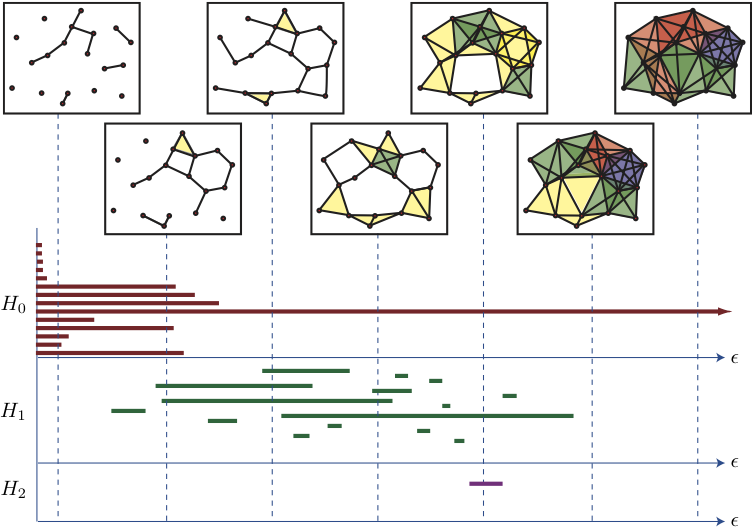
\includegraphics[width=0.75\textwidth]{barcode.png}\\
		\caption{Баркод}
		%\emph{Рис. 2. Баркод}
		\label{barcode}
	\end{center}
\end{figure}
\newline
Эту же информацию можно закодировать в виде диаграммы персистентности (рис. \ref{persist_diag}). Она строится следующим образом: каждый интервал баркода имеет начало $t_{birth}$ и конец $t_{death}$. На персистентной диаграмме каждый интервал баркода изображается в виде точки с координатами ($t_{birth}, t_{death}$), и каждая такая точка соответствует одному из слагаемых $I_{[j_k, s_k]}$ и $I_{[r_k, \infty)} $ из разложения. Чем дальше точка на персистентной диаграмме от диагонали, тем она важнее -- эта точка сигнализирует о наличии "$n$-мерной дырки". 
\begin{figure}[]
	\begin{center}
		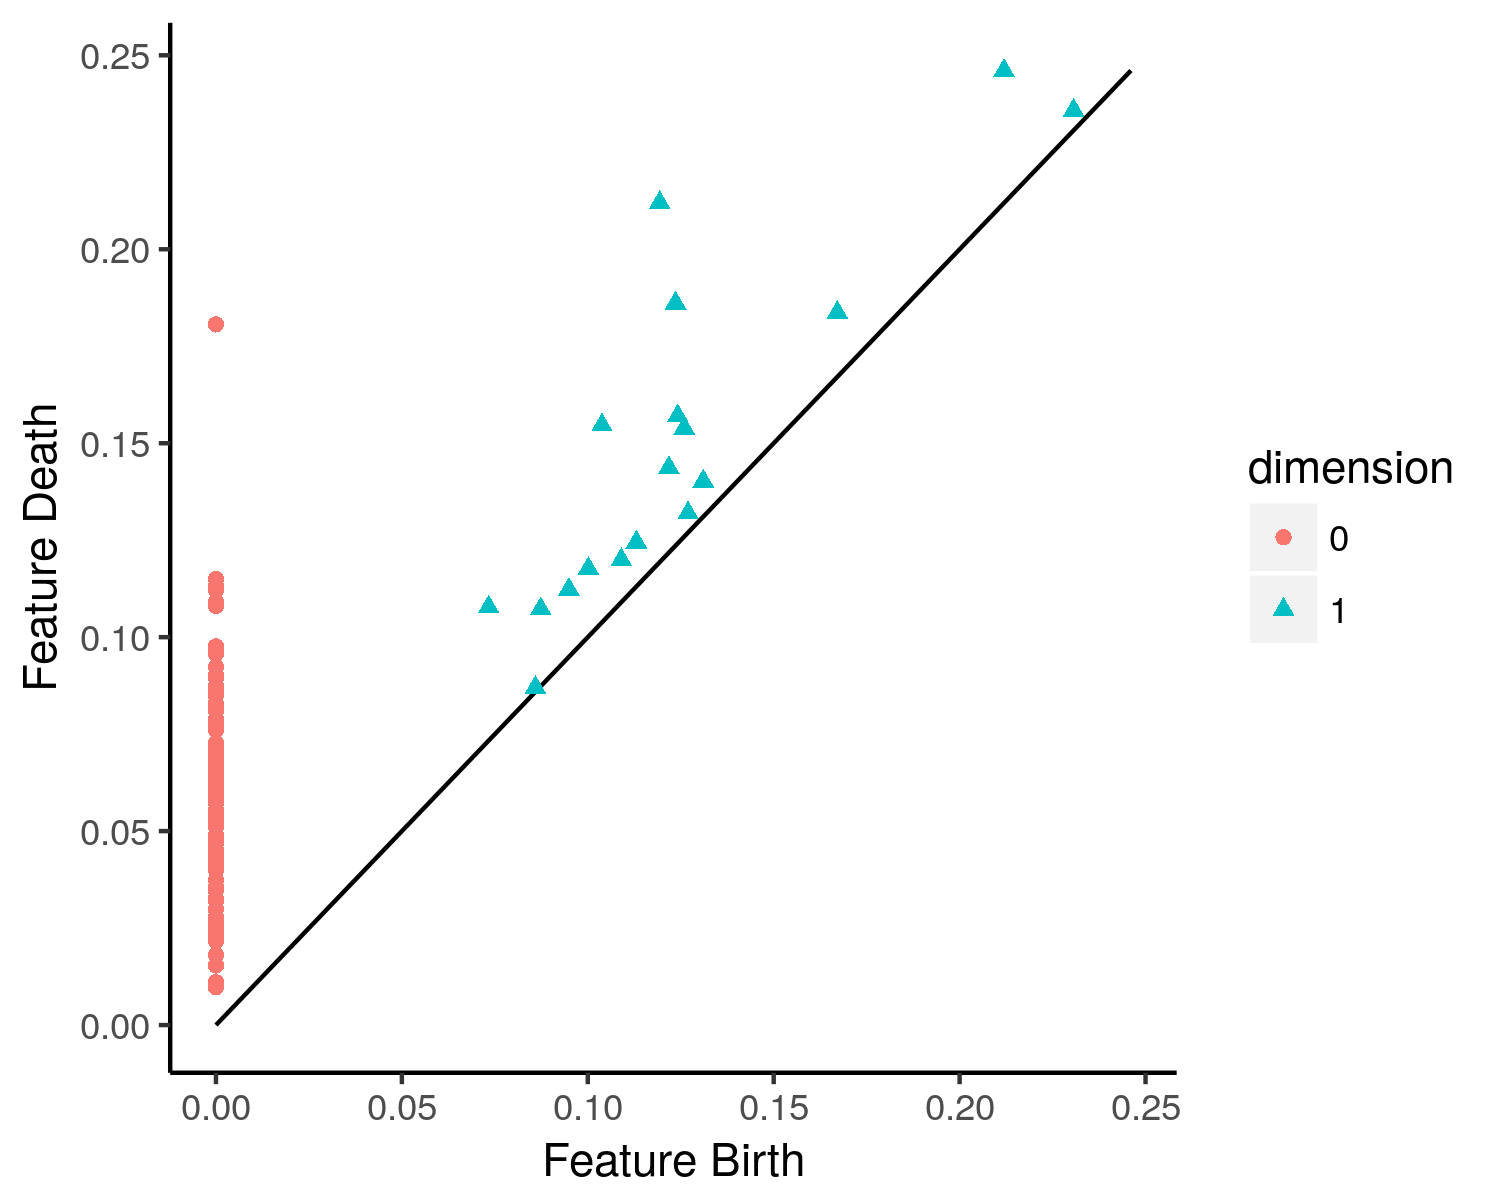
\includegraphics[width=0.6\textwidth]{persist_diag.png}\\
		\caption{Персистентная диаграмма}
		%\emph{Рис. 3. Персистентная диаграмма}
		\label{persist_diag}
	\end{center}
\end{figure}